\documentclass[10pt,aspectratio=169]{beamer}

% All the boilerplate is in deslides.sty
\usepackage{deslides}

\author{Ji\v{r}\'i Lebl}

\institute[OSU]{%
Oklahoma State University%
%Departemento pri Matematiko de Oklahoma {\^S}tata Universitato%
}

\title{7. Linear equations and the integrating factor\\(Notes on Diffy Qs, 1.4)}

\date{}

\begin{document}

\begin{frame}
\titlepage

%\bigskip

\begin{center}
The textbook: \url{https://www.jirka.org/diffyqs/}
\end{center}
\end{frame}

\begin{frame}
An first order equation is \emph{linear} if it is of the form
\[
y' + p(x) y = f(x)
\]
\pause
That is, linear in $y$ and $y'$.
\pause
Dependence on $x$ can be more complicated.

\medskip
\pause

Linear equations are quite well-behaved,
\pause
are easy to solve,
\pause
and are quite common.

\medskip
\pause

Trick is to multiply by some $r(x)$ to make the left hand side look like
\[
r(x) y' + r(x) p(x) y = \frac{d}{dx}\Bigl[ r(x) y \Bigr]
\]
\pause
If we have such an $r$, then the equation is
\[
\frac{d}{dx}\Bigl[ r(x) y \Bigr] = r(x)f(x)
\]
\pause
Integrate both sides, and solve for $y$:
\[
y = \frac{1}{r(x)} \left( \int r(x)f(x) \, dx + C \right)
\]
\pause
$r(x)$ is called the \emph{integrating factor}.
\pause
\qquad
That's all great but ... \pause What is $r(x)$?
\end{frame}

\begin{frame}
We want $r(x)$ so that $r'(x) = r(x)p(x)$:
\pause
\[
r(x) = e^{\int p(x) \,dx}
\]
\pause
We compute:
\begin{align*}
\uncover<3->{y' + p(x) y &= f(x) \\}
\uncover<4->{e^{\int p(x) \,dx} y' + e^{\int p(x) \,dx} p(x) y
  & = e^{\int p(x) \,dx} f(x) \\}
\uncover<5->{\frac{d}{dx}\left[ e^{\int p(x) \,dx} y \right]
  & = e^{\int p(x) \,dx} f(x) \\}
\uncover<6->{e^{\int p(x) \,dx} y
  & = \int e^{\int p(x) \,dx} f(x) \,dx + C \\}
\uncover<7->{y
  & = e^{-\int p(x) \,dx} \left( \int e^{\int p(x) \,dx} f(x) \,dx + C \right)}
\end{align*}
\end{frame}

\begin{frame}
\textbf{Example:}
Solve
\qquad
$\displaystyle
y' + 2xy = e^{x-x^2}, \qquad y(0) = -1$

\medskip
\pause

So $p(x) = 2x$ and $f(x) = e^{x-x^2}$

\medskip
\pause

The integrating factor is $r(x) = e^{\int p(x)\, dx} = e^{x^2}$.
\pause
\quad
Compute:
\begin{align*}
\uncover<4->{e^{x^2} y' + 2xe^{x^2}y
  & = e^{x-x^2} e^{x^2} \\}
\uncover<5->{\frac{d}{dx} \left[ e^{x^2} y \right]
  & = e^x \\}
\uncover<6->{e^{x^2} y
  & = e^x +C \\}
\uncover<7->{y 
  & = e^{x-x^2} + C e^{-x^2}}
\end{align*}
\uncover<8->{%
Solve for the initial condition: $-1 = y(0) \pause = 1 + C$, \pause so $C=-2$.

\medskip
}

\uncover<9->{%
So
\[
y = e^{x-x^2} - 2 e^{-x^2}
\]
}

\end{frame}

\begin{frame}
\textbf{Remark 1:}
Pick any antiderivative for $e^{\int p(x) dx}$, no need to put in a constant
of integration.

\medskip
\pause

\textbf{Remark 2:} I find it is easiest to remember just the formula for
$r(x)$ and how to repeat the process instead of memorizing the final
formula.

\medskip
\pause

\textbf{Remark 3:}
Can't always solve in closed form.  A formula with
a definite integral is useful.

\pause
\medskip

Consider \quad $y' + p(x) y = f(x) , \quad y(x_0) = y_0$.

\medskip
\pause

We have an explicit formula for the solution:
\[
y(x) = e^{-\int_{x_0}^x p(s)\, ds} \left( \int_{x_0}^x e^{\int_{x_0}^t p(s)\, ds}
f(t) \,dt + y_0 \right) \tag{$*$}
\]
\pause
Note all the ``dummy'' variables to write it correctly.

\medskip
\pause

\textbf{Exercise:}
Write the solution of
\quad $y' + y = e^{x^2-x}, \quad y(0) = 10$ \quad as
a definite integral

(no closed form solution exists).

\medskip
\pause

\textbf{Remark 4:}
There is a stronger version of Picard's theorem for linear equations:
\pause
Formula ($*$) says that if $f(x)$ and $p(x)$ are
continuous on an interval $(a,b)$, the solution also
exists and is continuous on $(a,b)$.
\pause
Nothing like that weird nonlinear $y'=y^2$ we saw before.
\end{frame}

\begin{frame}

\textbf{Example:}
A 100L tank contains 10kg of salt dissolved in 60L of water.

Brine (water and salt) of concentration 0.1\unitfrac{kg}{L}
flows in at 5\unitfrac{L}{min}.

The tank is well stirred and solution flows out at 3\unitfrac{L}{min}.

\vspace*{-0.45in}
\hspace*{4.5in}\scalebox{0.8}{\subimport{../figures}{lin-tank.pdf_t}}

\vspace*{-1.04in}

\pause
How much salt is in the tank when the tank is full?

\medskip
\pause

Let $x =$ kg of salt in tank.
\pause
Let $t$ be time in minutes.

\medskip
\pause

For small change $\Delta t$ in $t$, $x$ changes approx.\ as

\medskip

\quad$\displaystyle
\Delta x \approx
(\text{rate in} \times \text{concentration in}) \Delta t - 
(\text{rate out} \times \text{concentration out}) \Delta t$

\medskip
\pause

Divide by $\Delta t$ and take the limit
$\Delta t \to 0$:

\medskip

\quad$\displaystyle
\frac{dx}{dt} =
(\text{rate in} \times \text{concentration in})  - 
(\text{rate out} \times \text{concentration out})$

\medskip
\pause

Here ~ rate in $=5$,
concentration in $ = 0.1$,
rate out $ = 3$,
concentration out $ = \frac{x}{\text{volume}} = \frac{x}{60+(5-3)t}$

\medskip
\pause
So
\[
\frac{dx}{dt} =
(5 \times 0.1)  - 
\left(3 \frac{x}{60+2t}\right)
\qquad
\pause
\text{or}
\qquad
\frac{dx}{dt} +
\frac{3}{60+2t} x
=
0.5
\]
\end{frame}

\begin{frame}
For $\frac{dx}{dt} + \frac{3}{60+2t} x = 0.5$, the integrating
factor is
\[
r(t) = \exp \left( \int \frac{3}{60+2t} dt  \right)
\pause
=
\exp \left( \frac{3}{2} \ln (60+2t) \right)
\pause
=
{(60+2t)}^{3/2} .
\]
\pause
Compute
\begin{align*}
\uncover<4->{{(60+2t)}^{3/2} \frac{dx}{dt} + {(60+2t)}^{3/2} \frac{3}{60+2t} x
  & = 0.5{(60+2t)}^{3/2} \\}
\uncover<5->{\frac{d}{dt}\left[ {(60+2t)}^{3/2} x \right]
  & = 0.5{(60+2t)}^{3/2} \\}
\uncover<6->{{(60+2t)}^{3/2} x
  & = \int 0.5{(60+2t)}^{3/2} dt +C \\}
\uncover<7->{ x & = {(60+2t)}^{-3/2}
  \int \frac{ {(60+2t)}^{3/2} }{2} dt +C{(60+2t)}^{-3/2} \\}
\uncover<8->{ x & =
  {(60+2t)}^{-3/2} \frac{1}{10}{(60+2t)}^{5/2} +C{(60+2t)}^{-3/2} \\}
\uncover<9->{ x & = \frac{60+2t}{10} +C{(60+2t)}^{-3/2} }
\end{align*}
\end{frame}

\begin{frame}
At $t=0$, $x=10$:
\quad
$10 = x(0) \pause = \frac{60}{10} +C{(60)}^{-3/2} \pause = 6 +C{(60)}^{-3/2}$
\wthus
\pause
$C=4 ({60}^{3/2}) \approx 1859.03$.

\pause
\medskip

\hfill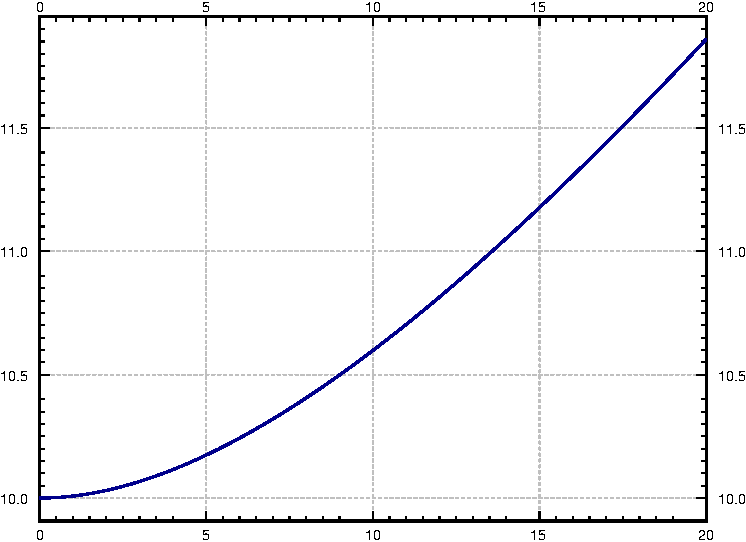
\includegraphics[height=1.8in]{../figures/linear-salt-graph}

\vspace*{-1.8in}

Here's a graph:

\medskip
\pause

So when is the tank full?

\pause
The tank is full when $60+2t = 100$, or $t=20$.

\medskip
\pause

What is $x$ when tank is full?

\medskip
\pause

\quad
$\displaystyle
x(20) = 
\frac{60+40}{10}
+C{(60+40)}^{-3/2}$

\quad
$\displaystyle
\phantom{x(20)}
\pause
\approx
10
+1859.03 {(100)}^{-3/2}
\approx
11.86
$

\medskip
\pause

The concentration when the tank is full is

approx.  $\nicefrac{11.86}{100} = \unitfrac[0.1186]{kg}{liter}$.

\medskip

(we started with $\nicefrac{1}{6}$ or \unitfrac[0.1667]{kg}{liter}.)

\end{frame}

\end{document}
